\section{Qualitative analysis}
Since PA measures during the weekdays and the weekend days are known to be different \cite{Watz_2009}, results were computed separately and only the ones relative to weekdays will be presented.
Figure~\ref{fig:10} illustrates the distribution of the dicovered routines $\beta_{1,..,18}$ over the terms of the vocabulary.
%% BETAS (DISTRIBUTION OVER THE WORDS)
\begin{figure}[ht!]
  \centering
  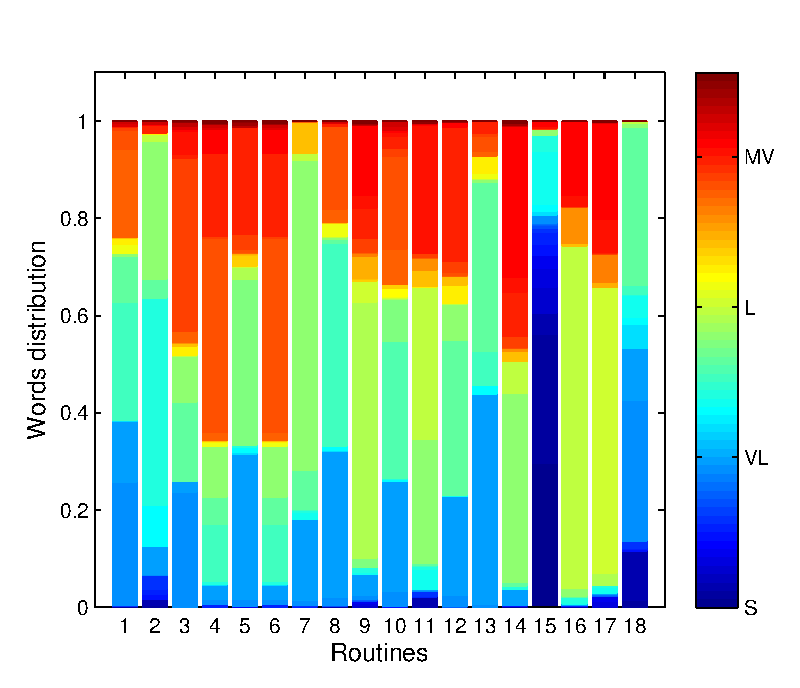
\includegraphics[width=.45\textwidth]{figure/eps/figure_10.eps}
  \caption[]{Distribution over the words}
  \label{fig:10}
\end{figure}
Four routines ($R2$, $R7$, $R13$, $R18$) related to low intensity levels, seven routines ($R4$, $R6$, $R9$, $R11$, $R14$, $R16$, $R17$) related high intensity levels and six routines ($R1$, $R3$, $R5$, $R8$, $R10$, $R12$) composed by a combination of VL, L and MV descriptors were discovered in data from 66 COPD patients and 66 healthy subjects. A separate routine ($R15$) characterizing the sleeping behavior was also found.
Each of these routines is characterized by a combination of words that in turn varies in relation to the feature levels. A detailed description of the routines with the 3 most important descriptors associated can be found in table~\ref{table:routines}. The words composing a particular routine are listed together with their occurrence probability (e.g. the first word of $R1$: \textit{[2 1 1 1]} refers to the descriptor \textit{$VL\_1^{d}\_1^{ST}\_1^{VM}$} and has an associated probability equal to 25\% ). Higher the probability, higher the importance of the descriptor for the routine.
%%%%%%%%%%%%%%%%%%%%%%%%%%%%%	TABLE RoutineS DISCOVERED	%%%%%%%%%%%%%%%%%%%%
%\newpage
%\begin{sidewaystable*}[H!]
%\centering
%\begin{tabular}{|c|c|c|c|c|c|c|c|c|c|c|c|c|c|c|c|c|c|c|c|}
%\hline
%Topic1  &    &  Topic2  &   &  Topic3  &    &  Topic4  &   & Topic5  &    &  Topic6  &    &  Topic7  &    &  Topic8  &    &  Topic9  &    &  Topic10  &	\\
%\hline
%\hline
%3 1 1 1  &  0.1  &  3 1 2 5  &  0.1  &  4 2 2 1  &  0.2  &  3 1 2 4  &  0.1  &  3 1 1 1  &  0.3  &  2 2 1 1  &  0.2  &  4 2 1 1  &  0.1  &  1 1 3 1  &  0.2  &  4 3 2 1  &  0.1  &  3 2 2 1  &  0.2  \\
%\hline
%4 1 2 1  &  0.1  &  4 1 2 1  &  0.1  &  3 1 2 4  &  0.1  &  2 2 2 1  &  0.1  &  3 1 1 4  &  0.1  &  1 1 2 1  &  0.2  &  3 1 1 1  &  0.1  &  2 1 1 2  &  0.1  &  2 1 2 3  &  0.1  &  3 2 1 1  &  0.1  \\
%\hline
%4 1 1 1  &  0.1  &  3 1 2 6  &  0.1  &  3 1 2 5  &  0.1  &  3 1 2 3  &  0.1  &  3 1 1 5  &  0.1  &  2 2 2 1  &  0.1  &  4 3 1 1  &  0.1  &  1 1 3 2  &  0.1  &  3 1 2 4  &  0.1  &  4 3 2 1  &  0.1  \\
%\hline
%2 1 2 3  &  0.1  &  2 1 2 5  &  0.1  &  2 1 2 4  &  0.1  &  3 1 2 2  &  0.1  &  2 1 2 4  &  0.0  &  2 1 1 2  &  0.1  &  2 1 1 6  &  0.0  &  3 1 1 1  &  0.1  &  3 1 2 3  &  0.1  &  3 2 2 3  &  0.0  \\
%\hline
%3 1 2 3  &  0.1  &  3 1 2 4  &  0.1  &  3 1 2 3  &  0.1  &  4 2 2 1  &  0.1  &  3 1 1 3  &  0.0  &  1 1 1 1  &  0.1  &  3 1 1 6  &  0.0  &  2 2 2 1  &  0.1  &  3 1 2 5  &  0.1  &  3 2 2 4  &  0.0  \\
%\hline
%3 1 2 2  &  0.0  &  2 1 2 6  &  0.1  &  2 1 2 3  &  0.1  &  4 2 2 3  &  0.0  &  3 1 1 6  &  0.0  &  1 1 2 2  &  0.0  &  3 1 1 7  &  0.0  &  1 2 3 1  &  0.0  &  3 1 2 2  &  0.1  &  2 1 2 3  &  0.0  \\
%\hline
%2 1 2 2  &  0.0  &  4 1 2 5  &  0.0  &  4 2 2 5  &  0.0  &  2 1 2 4  &  0.0  &  2 1 1 4  &  0.0  &  1 1 1 2  &  0.0  &  3 1 1 5  &  0.0  &  3 1 2 4  &  0.0  &  2 1 2 4  &  0.0  &  3 2 2 5  &  0.0  \\
%\hline
%3 1 1 4  &  0.0  &  3 1 2 7  &  0.0  &  3 1 2 6  &  0.0  &  4 2 2 2  &  0.0  &  3 1 2 4  &  0.0  &  3 1 1 6  &  0.0  &  4 1 1 1  &  0.0  &  2 1 2 2  &  0.0  &  2 1 2 2  &  0.0  &  2 1 2 4  &  0.0  \\
%\hline
%2 1 2 4  &  0.0  &  4 1 2 6  &  0.0  &  4 2 2 4  &  0.0  &  3 1 2 5  &  0.0  &  3 1 2 5  &  0.0  &  3 1 1 5  &  0.0  &  3 1 1 3  &  0.0  &  2 2 1 1  &  0.0  &  3 1 2 6  &  0.0  &  4 2 2 1  &  0.0  \\
%\hline
%3 1 2 4  &  0.0  &  3 1 2 3  &  0.0  &  2 1 2 2  &  0.0  &  2 1 2 3  &  0.0  &  2 1 1 5  &  0.0  &  1 2 2 1  &  0.0  &  2 1 2 6  &  0.0  &  3 1 2 5  &  0.0  &  4 3 2 5  &  0.0  &  3 2 2 2  &  0.0  \\
%\hline
%3 1 1 3  &  0.0  &  4 1 2 4  &  0.0  &  3 1 1 1  &  0.0  &  2 2 1 1  &  0.0  &  2 2 1 1  &  0.0  &  3 1 1 7  &  0.0  &  4 2 2 1  &  0.0  &  1 1 2 1  &  0.0  &  4 3 2 4  &  0.0  &  2 1 2 2  &  0.0  \\
%\hline
%4 1 2 4  &  0.0  &  2 2 2 1  &  0.0  &  3 1 2 2  &  0.0  &  4 1 2 1  &  0.0  &  2 1 2 3  &  0.0  &  2 1 2 2  &  0.0  &  3 1 1 4  &  0.0  &  3 1 2 6  &  0.0  &  3 1 1 1  &  0.0  &  3 2 1 4  &  0.0  \\
%\hline
%3 1 1 5  &  0.0  &  3 1 1 6  &  0.0  &  4 2 2 6  &  0.0  &  4 2 2 4  &  0.0  &  2 1 2 5  &  0.0  &  3 1 2 6  &  0.0  &  4 2 1 7  &  0.0  &  3 1 2 3  &  0.0  &  2 1 2 5  &  0.0  &  3 2 2 6  &  0.0  \\
%\hline
%3 1 1 2  &  0.0  &  3 1 1 1  &  0.0  &  2 1 2 5  &  0.0  &  4 3 2 2  &  0.0  &  2 1 1 3  &  0.0  &  3 1 1 1  &  0.0  &  4 2 1 6  &  0.0  &  3 1 1 4  &  0.0  &  3 1 2 7  &  0.0  &  3 2 1 5  &  0.0  \\
%\hline
%4 1 2 3  &  0.0  &  2 1 2 4  &  0.0  &  4 2 2 3  &  0.0  &  4 3 2 3  &  0.0  &  3 1 2 3  &  0.0  &  1 2 1 1  &  0.0  &  3 1 1 2  &  0.0  &  3 1 1 6  &  0.0  &  4 3 2 3  &  0.0  &  3 2 1 3  &  0.0  \\
%\hline
%\end{tabular}
%\caption{Topics words-probabilities (04 002 means the second word of intensity 4}
%\label{table:Table 7}
%\end{sidewaystable*}

\begin{table}[ht!]
\centering
\scalebox{0.65}{
\begin{tabular}{|c|c|c|c|c|c|c|c|c|c|c|c|}
\hline
R1  & \%   &  R2  & \%  &  R3  &  \%  &  R4  &  \% & R5  &   \%  & R6  &   \% \\
\hline
\hline
2 1 1 1  &  0.25  &  2 2 2 2  &  0.43  &  4 1 2 1  &  0.36  &  4 1 1 2  &  0.40  &  3 1 2 2  &  0.34  &  4 1 1 2  &  0.40  \\
\hline
3 1 1 1  &  0.24  &  3 1 3 1  &  0.28  &  2 1 1 1  &  0.24  &  4 1 2 2  &  0.17  &  2 1 1 2  &  0.30  &  4 1 2 2  &  0.17  \\
\hline
4 1 1 1  &  0.18  &  2 2 1 2  &  0.09  &  3 1 2 1  &  0.16  &  3 1 1 1  &  0.12  &  4 1 2 2  &  0.22  &  3 1 1 1  &  0.12  \\
\hline
\hline
R7  &  \% &  R8  &  \%  &  R9  & \%  & R10  &  \%  & R11  &  \%  & R12  &   \% \\
\hline
\hline
3 1 3 1  &  0.64  &  3 1 1 1  &  0.42  &  3 1 3 2  &  0.53  &  3 1 1 2  &  0.28  &  3 1 4 1  &  0.31  &  3 1 2 1  &  0.32  \\
\hline
2 1 1 2  &  0.17  &  2 1 1 2  &  0.30  &  4 1 3 2  &  0.15  &  2 1 1 2  &  0.23  &  4 1 3 1  &  0.26  &  4 1 2 2  &  0.28  \\
\hline
3 1 2 1  &  0.08  &  4 1 1 2  &  0.17  &  4 1 2 2  &  0.06  &  4 1 1 2  &  0.19  &  3 1 3 1  &  0.25  &  2 1 1 2  &  0.20  \\
\hline
\hline
R13  &  \% &  R14  &  \%  &  R15  & \%  & R16  &  \%  & R17  &  \%  & R18  &   \% \\
\hline
\hline
2 1 1 2  &  0.43  &  3 1 3 1  &  0.39  &  1 1 1 1  &  0.30  &  3 1 4 1  &  0.70  &  3 1 4 2  &  0.59  &  3 1 2 1  &  0.32  \\
\hline
3 1 2 1  &  0.35  &  4 1 3 2  &  0.31  &  1 1 1 2  &  0.27  &  4 1 3 2  &  0.15  &  4 1 3 2  &  0.20  &  2 1 1 1  &  0.29  \\
\hline
3 1 1 1  &  0.07  &  4 1 2 2  &  0.09  &  2 2 2 1  &  0.11  &  3 2 4 1  &  0.07  &  4 1 3 1  &  0.07  &  2 1 1 2  &  0.11  \\
\hline
\end{tabular}
}
\caption{Routines matrix}\label{table:routines}
\end{table}
%
Figure~\ref{fig:12} illustrates the activation probability of the extracted routines when day segments of 30 minutes are sequentially inferred. The top plot and the bottom plot show respectively the routine patterns for a COPD patient and a healthy subject. It can be seen that 3 PA routines ($R2$, $R3$ and $R15$) pervade the day of a COPD patient~(top plot of Fig.~\ref{fig:12}). In particular this patient spent most of his time performing activities that involve a VL intensity descriptor of long duration, with high $\mu_{ST}$ and high $\mu_{VM}$ and a L intensity descriptor of short duration, with high $\mu_{ST}$ and low $\mu_{GSR}$. After 5 hours from the patient awakening we can see that $R13$ becomes dominant for 1 hour. This routine includes a VL descriptor of short duration, small $\mu_{ST}$ and high $\mu_{VM}$, and a L intensity descriptor of short duration, medium-low $\mu_{ST}$ and low $\mu_{GSR}$. It can also be seen that around 12 hours after the awakening of the subject $R12$ starts decreasing and $R15$, characterizing the sleeping behavior, starts to become the most active routine. On the other hand the day of a healthy subject shows a more variety of active routine patters. It can be seen from the bottom plot of Fig.~\ref{fig:12} that in the first phase of the day an alternating sequence of the routines $R13$ and $R12$ is present. $R12$ in particular is composed by descriptors related to L and MV intensities of short duration, medium-low $\mu_{ST}$ and low $\mu_{GSR}$. Around 5 hours after his awakening and in the evening before sleeping this subject assumes a similar behavior if compared to his COPD match. In particular, first routine $R12$ becomes the dominant routine for about 1 hour, and then it is active permanently until the sleeping time.
%
%
%
%
\begin{figure*}[ht]
  \centering
  \mbox{\subfloat{\label{fig:12a} 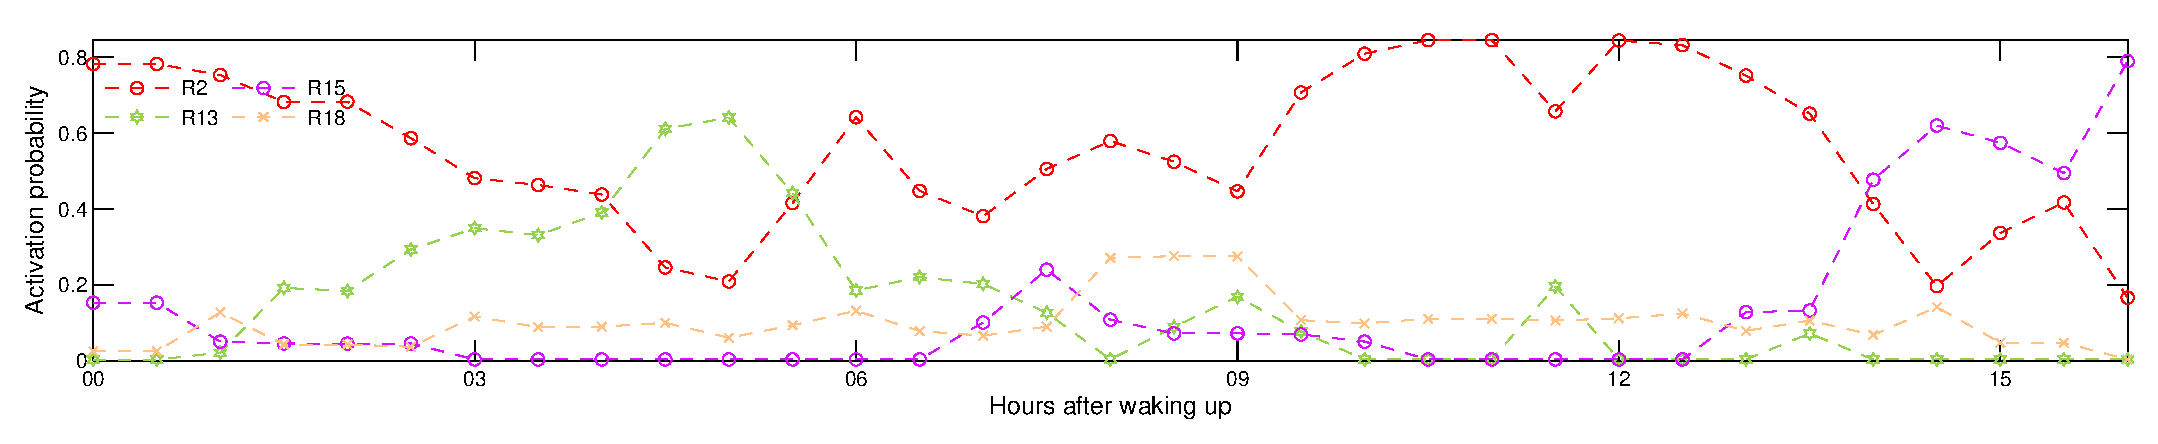
\includegraphics[width=.9\textwidth, height=3cm]{figure/eps/figure_4_1_copd_weekday.eps}}}
  \mbox{\subfloat{\label{fig:12b} 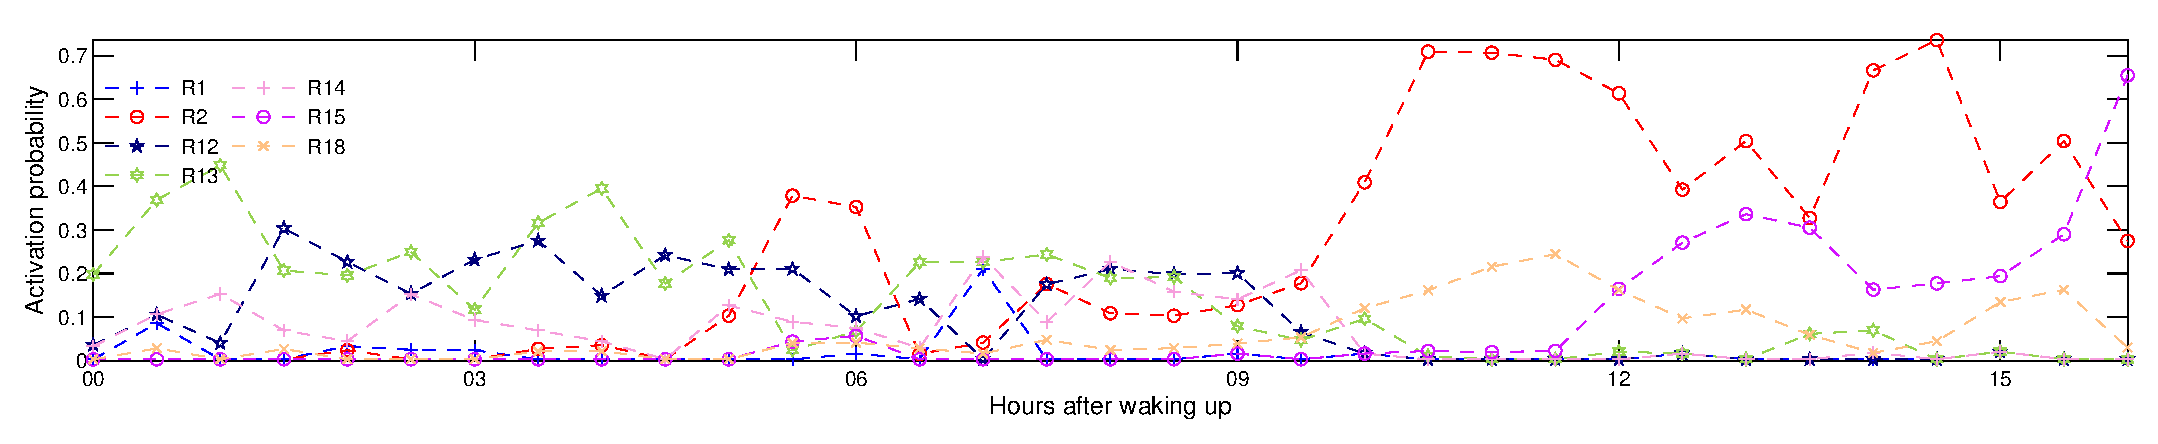
\includegraphics[width=.9\textwidth, height=3cm]{figure/eps/figure_4_1_healthy_weekday.eps}}}
  \caption{Routines found inferring a COPD patient day (top) and a healthy subject (bottom). Only topics reaching an activation $>0.2$ are shown.}\label{fig:12}
\end{figure*}
%
%
The  validity and robustness of the routines estimated are qualitatively highlighted in Fig.~\ref{fig:6}. Indeed, the routines discovered on a sub-sample of 66 patients were also inferred in the same way on data from 977 patients showing similar patterns. We can see that, on average, for COPD patients the PA descriptor $R2$ is almost always active across the days. This is consistent with other studies showing physical inactivity in patients with COPD~\cite{Troosters_2010}.
\begin{figure*}[ht]
  \centering
  \mbox{\subfloat[66 COPD patients.]{\label{fig:6a} 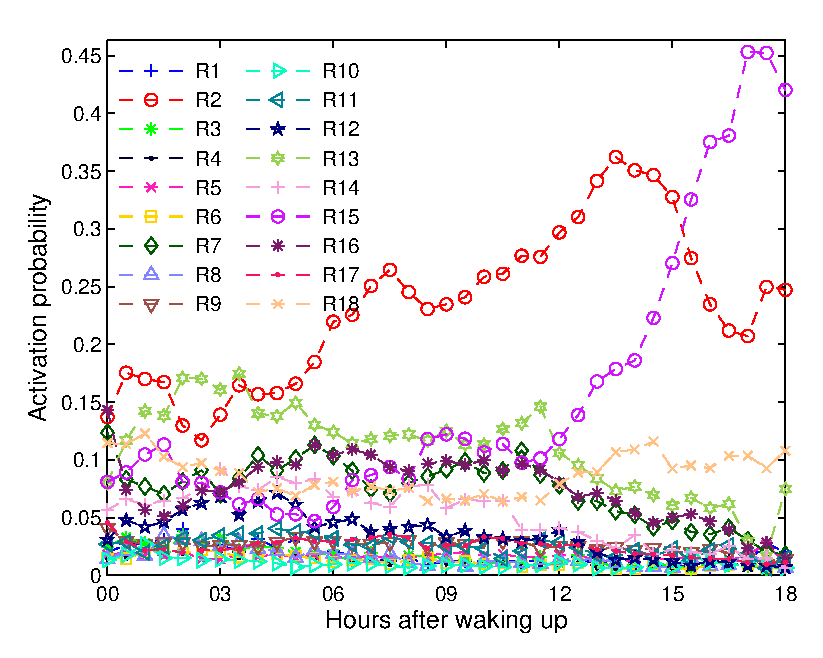
\includegraphics[width=.45\textwidth]{figure/eps/figure_4_copd_weekday.eps}}}
  \mbox{\subfloat[977 COPD patients.]{\label{fig:6b} 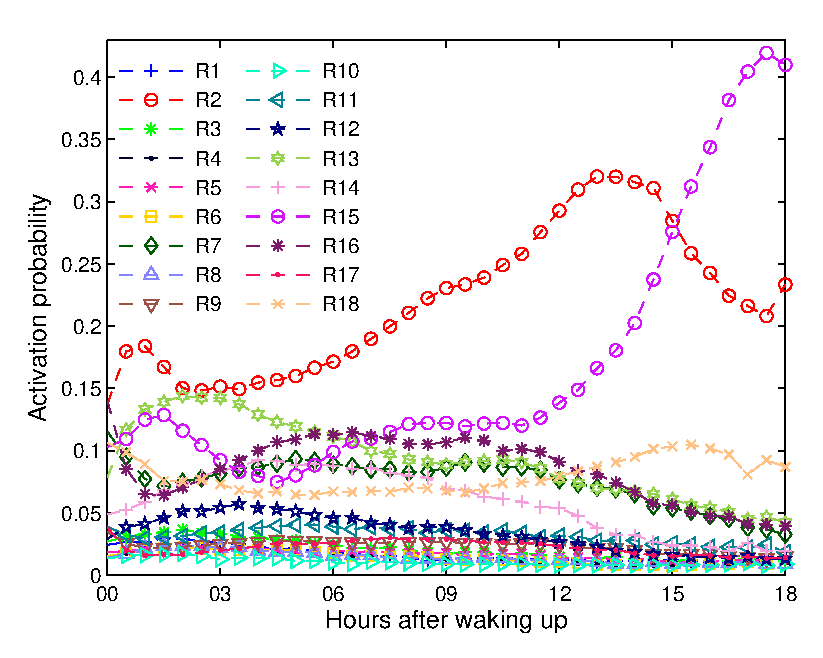
\includegraphics[width=.45\textwidth]{figure/eps/figure_4_patients_weekday.eps}}}
    \caption{Routines found inferring days from 66 COPD patients (left) and a 977 COPD patients (right). The figures show the average activation probability across the patients samples.}\label{fig:6}
\end{figure*}
%
%
Fig.~\ref{fig:7_mean} shows the average values of the routines' activation probabilities when the inference is performed on the first 6 hours after the subjects awakenings. Subjects were stratified according to their disease severity where GOLD1 and GOLD4 indicates respectively the least and most severe stage of COPD. Each point identifies the mean across all the subjects belonging to one of the 4 categories. Healthy subjects formed a separated category. 
We can observe that routines are organized according to COPD severity. In particular we can observe 4 main trends. $R2$ and $R15$ are increasing with the increase of COPD severity. In particular $R2$ represents a medium-inactive PA routine composed for the 43\% by $VL\_2^{d}\_2^{ST}\_2^{VM}$ and for the 28\% by $L\_1^{d}\_3^{ST}\_1^{GSR}$. The first PA descriptor represents very light intensity movements that cause a moderate increase of the temperature and that last for a long duration. The second descriptor represent light intensity movements characterized by short duration and a high physiological response (high body temperature). The positive trend is interrupted in the most severe group of patients that compensate a smaller value for $R2$ with a higher value of $R16$. This PA routine is characterized from PA descriptors including $L$ and $MV$ intensities and characterized by higher physiological responses if compared to $R2$. This might indicate a bigger effort in performing activities.
Another positive trend is shown by $R15$ representing the time spent while performing a very inactive behavior (mainly sleeping).
On the other hand we can note that $R13$, $R12$ and $R1$ decrease with an increase in COPD severity. These 3 routines indicate movements performed with medium ($R13$) and high ($R1$ and $R12$) activity intensities characterized by small physiological responses.
%
\begin{figure}[ht]
  \centering
%  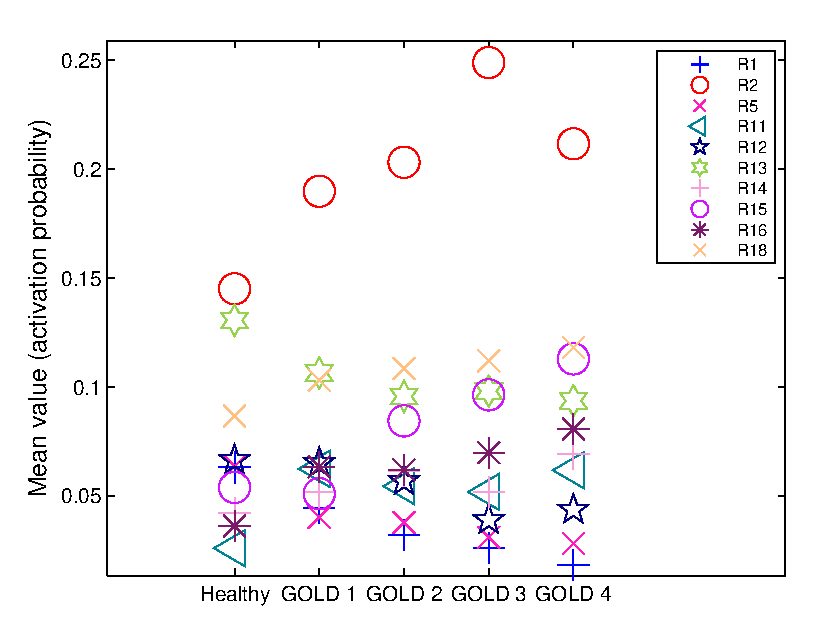
\includegraphics[width=.45\textwidth]{figure/eps/figure_7_trend_all_weekday.eps}
  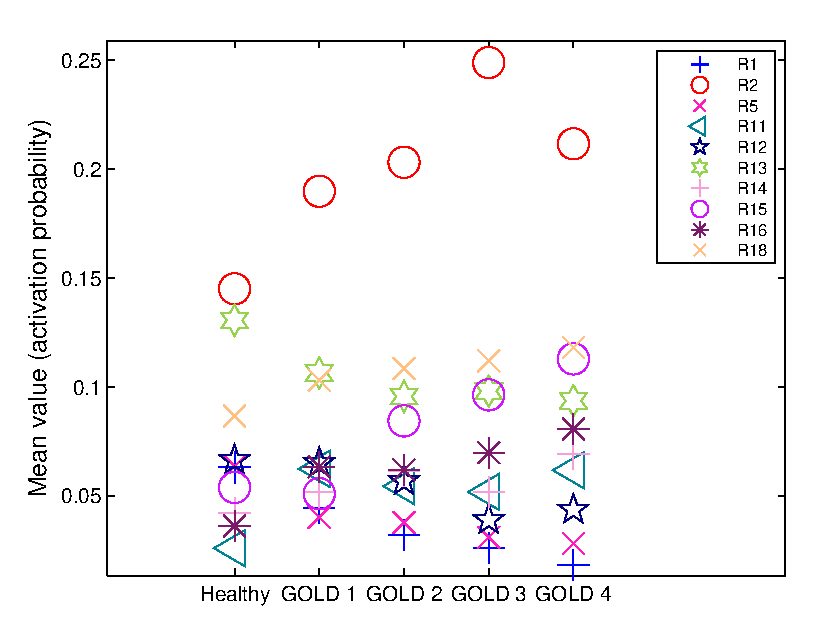
\includegraphics[width=.45\textwidth]{figure/eps/figure_7_trend_all_weekday.eps}
  \caption[]{Activation topic averages after stratification for COPD severity across 6h weekday. Inference was performed in the first 6 hours after the awakenings from the night sleep.}
  \label{fig:7_mean}
\end{figure}
Of particular interest are $R1$ and $R13$ since they are weakly but significantly correlated with $FEV_{1},\%predicted$ ($\rho=0.2$, $p=4e^{-10}$ and $\rho=1.8$, $p=1.84e^{-8}$ respectively). No correlation was found with BMI and age for $R1$. $R13$ is weakly correlated with age ($\rho=-0.18$, $p=5.3e^{-9}$). Differently from other results in literature where PA measures were highly correlated with BMI, the routines discovered seems to be decoupled from it and, although a more detailed analysis is necessary, they seem reflecting the stage of the disease as measured by common clinical practice.
In more, performing ANOVA test statistical differences have been found in the percentage of activation of $R1$ between GOLD1, GOLD3 and GOLD4 and between GOLD2 and GOLD4. Regarding $R13$ statistical differences have been found between GOLD1, GOLD3 and GOLD4, and between GOLD2, GOLD3 and GOLD4.

